\chapter{Background}
\label{chap:bg}

\section{Basic Concepts}
\label{sec:concepts}
\subsection{Affective Computing and Affect Control Theory}

Affective Computing refers to the study of developing machines (or computer programs) capable of recognizing, interpreting, processing and generating human affect. It is an interdisciplinary field spanning computer science, psychology, and cognitive science, and is believed to be an important topic for ``harmonious human-computer interaction'' \cite{tao2005affective}. One aspect that Artificial Intelligence (AI) researchers have recently been concerned about is to have machines interact with humans emotionally. That is to say, machines should interpret the emotional state of humans and adapt its behaviours to them, i.e. to give appropriate responses for those emotions. With the ability to process affective information, machines are believed to exhibit higher flexibility, and to work in uncertain or complex environments \cite{picard2000affective}.

Affective computing research is based on theories of emotion \cite{lewis2010handbook}. Among all the popular emotions theories proposed, two main representations of emotional or affective states are used: categorical labels, and dimensional models. Based on their linguistic use in daily life, categorical labels can be used to describe affective states. Different set of labels can be chosen depending on the study. Most frequently, the following labels are used to describe affective states: anger, happiness, sadness, surprise, disgust and fear \cite{ekman1992there}. Dimensional models represent affective states as vectors containing a set of independent dimensions. The value for each of the dimensions can be real numbers. A common set of dimensions used to capture emotional experiences in researches consists of three factors \cite{scholl2013socio}. The first one is variously called friendliness-hostility, pleasure, valence, describing a general positive versus negative evaluation of the emotional experience. The second is alternatively called dominance-submissiveness, control, power, or potency. It captures the amount of control over others and the surroundings versus feeling controlled by external circumstances. The third one is interchangeably called activation, arousal, and activity. Activity level corresponds to the level of activation, mental alertness, and physical activity. A fourth dimension relating to the ``uncertainty'' of situations is also proposed by some research \cite{fontaine2007world}.  Compared with categorical labels, dimensional representations may relate more to the underlying physiological changes \cite{mauss2009measures}.

One well known sociological theory that describes emotions as three-dimensional vector that represents evaluation ($E$), potency ($P$), and activity ($A$) respectively is Affect Control Theory (ACT) \cite{robinson2006affect}. Different from categorical labels, the EPA-vector representation describes affective meanings of concepts in precise, measurable ways. By using the same three affective scales, programs implemented based on ACT are able to track the affective meanings of actors and behaviours in an interaction.

ACT describes social events by an Actor-Behaviour-Object (ABO) grammar: \textit{Actor Behaves} towards \textit{Object}, where Object is usually another actor (e.g. a human). Each of the ABO elements is associated with an EPA vector. The EPA values of the interactants' identities, behaviours, and environmental settings are referred to fundamental sentiments in ACT. ACT hypotheses that the fundamentals of identities, behaviours, etc, are shared between people within a same culture. On the other hand, the emotional feelings of people evoked by a specific event are referred as transient impressions, and can be measured by in-context ratings of the ABO elements. ACT proposes that people behave in interactions to minimize the deflection of transient impressions to fundamental sentiments. This proposition is referred to as the Affect Control Principle defined below.

\newtheorem{def-act}{Definition}
\begin{def-act}
\label{def:act}
The Affect Control Principle \cite{robinson2006affect}: Actors work to experience transient impressions that are consistent with their fundamental sentiments.
\end{def-act}

The ACT hypothesis that fundamentals are shared within same culture is supported with a large variety of studies. Tests of ACT's validity on both verbal (e.g. INTERACT) and non-verbal behaviours \cite{schroder2013culture} have been reported. EPA profiles of concepts, including identities and behaviours, can be measured with the semantic differential, a survey technique where respondents rate affective meanings of concepts on numerical scales. In general, within-cultural agreement about EPA meanings of social concepts is high even across subgroups of society, and cultural-average EPA ratings from as little as a few dozen survey participants are extremely stable over extended periods of time. For example, the EPA for the identity of ``nurse'' is $[1.65, 0.93, 0.34]$, meaning that nurses are seen as quite good, a bit powerful, and a bit active. Comparatively a ``patient'' is seen as $[0.9, -0.69, -1.05]$, less powerful and active than a ``nurse''.

With the hypothesis that people within same culture share the same expectations, or fundamental sentiments, for each identity and action, ACT proposes that the two communicating parties sharing the same cultural background would act to minimize deflections from fundamental sentiments during interactions. If a large deflection is caused for some reason, they choose actions that can restore the impression. ACT implies that the two communicating parties, knowing or having beliefs about their identities, would not only have expectations on what they should perform in the interaction, but would also have expectations on what the other party should perform. For example, in a situation where a student is asking a tutor questions and both of them are aware of their identities, the student is supposed to be polite, less powerful and more active, while the tutor is supposed to be patient, more powerful and less active. The interaction would go smoothly if the tutor performs these expected actions, e.g. answers the student's questions patiently. However, if the tutor suddenly yells at the student criticizing him/her for being stupid, a large deflection would be caused. The student's focus would shift from solving his/her previous problems; he/she would start to figure out why he/she was yelled and what he/she should perform to have the tutor become nicer.

ACT can serve as a general psychological principle of micro-regulation of interpersonal interactions. By presenting all affective meanings as three-dimensional vectors, i.e. the EPA vectors, it enables mathematical computations on past sentiment interactions and thus presents a maximum likelihood solution predicting optimal behaviours or identities. 

\subsection{POMDP}


\begin{figure}[htb]
\centering
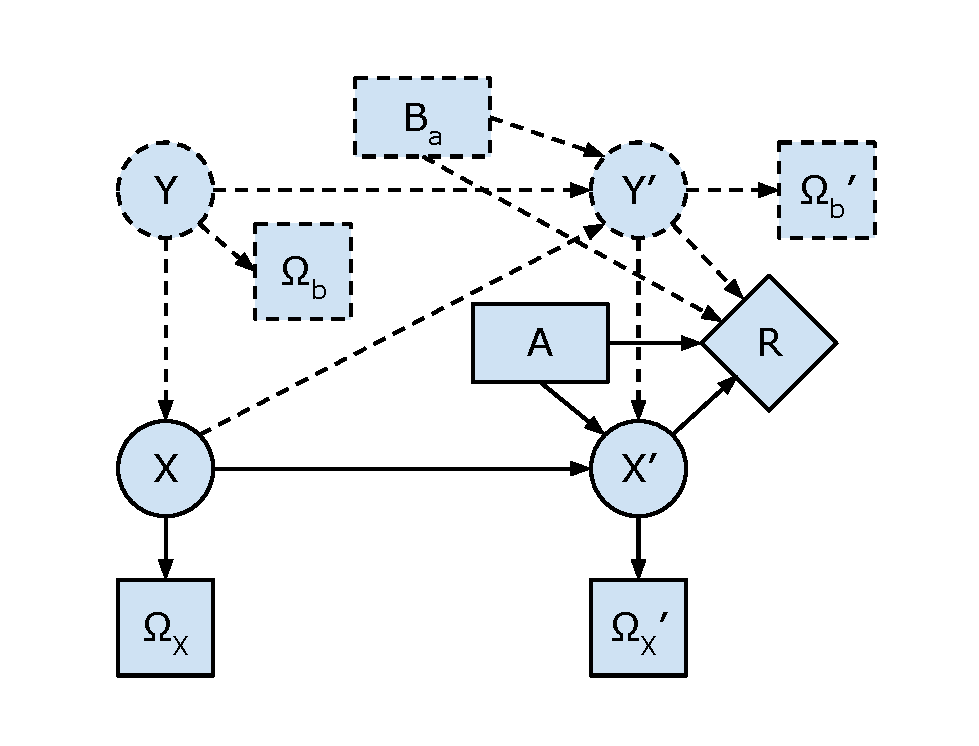
\includegraphics[trim = 10mm 10mm 10mm 10mm, clip, width=0.6\linewidth]{fig/fig-pomdp.pdf}
\caption{A time slice of a general POMDP (solid lines) and a POMDP augmented with affective states (dotted lines)}
\label{fig:pomdp}
\end{figure}

A partially observable Markov decision process (POMDP) is a general stochastic model that has been extensively studied in operations research and in artificial intelligence \cite{monahan1982state, poupart2011introduction}. Figure~\ref{fig:pomdp} shows a time slice of a general POMDP (solid lines). Capital symbols (e.g. $X$) are used to denote variables or features, small symbols (e.g. $x$) are to denote values of these variables, and boldface symbols (e.g. $\mathbf{X}$) are to denote sets of variable values. Primes are used to denote post-action variables, so $x'$ means the value of the variable $X$ after a single time step. As shown in the figure, a POMDP consists of a finite set $\mathbf{X}$ of states $X$; a finite set $\mathbf{A}$ of actions $A$; a stochastic transition model $Pr : X \times A \to \Delta(\mathbf{X})$, where $Pr(x'|x, a)$ denotes the probability of moving from state $x$ to $x'$ after an action a is taken, and $\Delta(\mathbf{X})$ is a distribution over $\mathbf{X}$, a finite observation set $\mathbf{\Omega_{X}}$, and a reward assigning function $R(A, X')$. The reward function $R(a, x')$ denotes the reward received to transit to $x'$ induced by action $a$. A stochastic observation model $Pr : X \to \Delta(\mathbf{\Omega_{X}})$ is used to denote the probability of making observation $\omega$ while the system is in state $x$. Basing on the aforementioned elements, a policy can be developed to map belief states (i.e. distributions over $X$) into choices of actions, such that the expected discounted sum of rewards is (approximately) maximized. POMDPs have been used as models for many human-interactive domains, including human assistance systems \cite{hoey2010automated}.

Figure~\ref{fig:pomdp} (dotted lines) shows a time slice of a general POMDP augmented with affective states. In addition to the basic POMDP elements, affective states $\mathbf{Y}$ are included in the POMDP process. $\mathbf{Y}$ describes the system's beliefs of the user's emotional states. Similarly to $\Omega_{X}$ and $A$, $\Omega_{b}$ denotes observations of user behaviours that gives the system evidence about state $Y$, and $B_{a}$ is the affective meaning of system action that can cause state $Y$ to change. Finally, the reward function $R(A, X', Y')$ is defined over state-action pairs and rewards those states and actions that are beneficial overall to the goals of the system-human interaction. 

\subsection{BayesACT}

ACT models interactions between two persons with a prerequisite that the identities of the two communicators are known to each other. This prerequisite has limited its usefulness in our application, where the user's identity is unpredictable. On the other hand, a Bayesian version of the ACT theory, called BayesACT, was formulated in Hoey et. al.'s work \cite{hoey2013bayesian}. This new model can maintain multiple hypotheses about identities and behaviours simultaneously as a probability distribution, and can make value-directed action choices. By employing BayesACT, machines are able to generate affectively believable interactions with people by learning about their identity, predicting their behaviours, and taking actions that are simultaneously goal-directed and affect-sensitive.

\begin{figure}[htb]
\centering
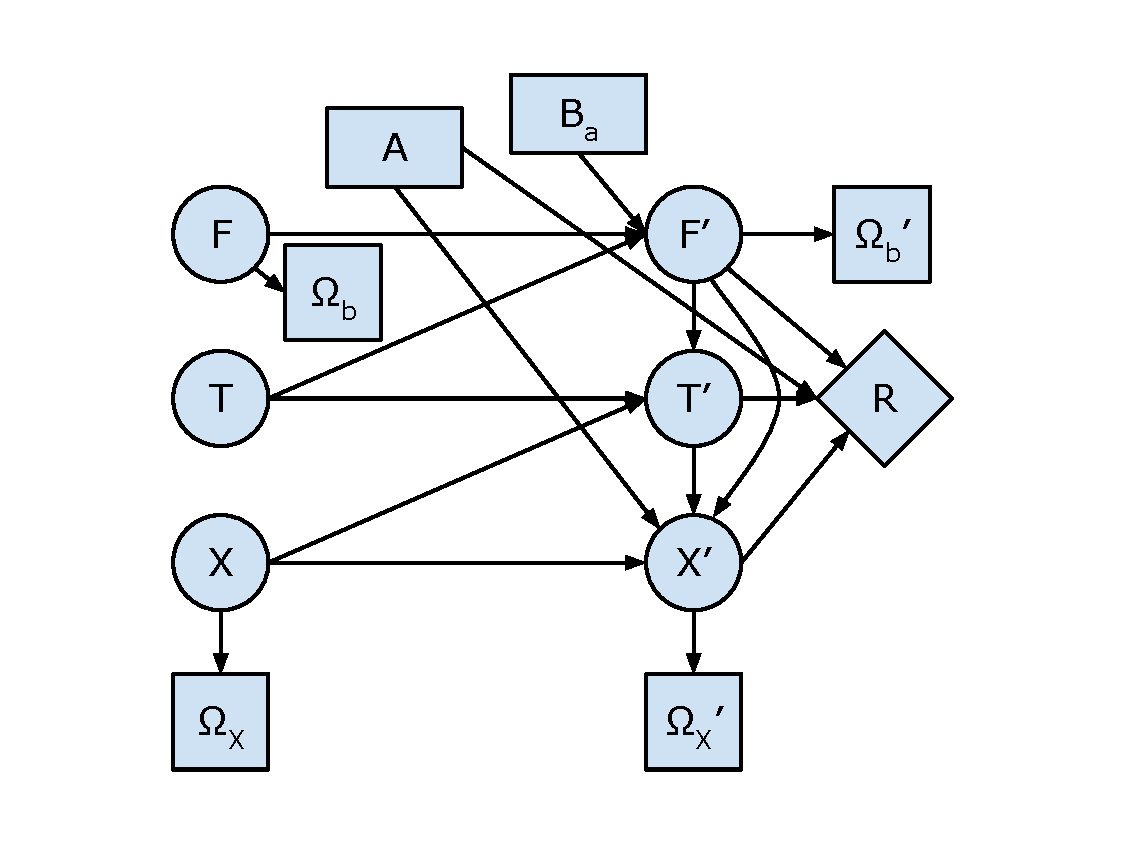
\includegraphics[trim = 10mm 10mm 10mm 10mm, clip, width=0.7\linewidth]{fig/fig-bayesact.pdf}
\caption{A factored POMDP for Bayesian Affect Control Theory}
\label{fig:bayesact}
\end{figure}

Figure~\ref{fig:bayesact} shows a factored POMDP for the BayesACT. It describes, from the perspective of the agent (although this is symmetric), how the variable state changes based on an interaction between an agent (i.e. a machine) and a client (i.e. a human). In our description of the figure, capital symbols (e.g. $F$, $T$) denote variables or features. Small symbols (e.g. $f$, $t$) denote values of these variables, and boldface symbols (e.g. $\mathbf{B_{a}}$) denote sets of variable values. Primes are used to denote post-action variables, so $x'$ means the values of the variable $X$ after a single time step.

In the figure, $X$ is used to represent everything the system needs to know about the system state, for example, the functional state of the agent and the client. To indicate which party acts at the given time step, $X$ encodes turn-taking messages as well. $F = \{F_{ij}\}$ denote the set of fundamental sentiments the agent holds, where each feature $F_{ij}, i \in \{a, b, c\}, j \in \{e, p, a\}$ denotes the $j$-th value of the $i$-th interaction object: $a$ (actor), $b$ (behaviour), or $c$ (client). Similarly, $T = \{T_{ij}\}$ is defined and denote the set of transient sentiment the agent holds. Variables $F_{ij}$ and $T_{ij}$ are continuous valued and $F$, $T$ are each vectors in a continuous nine-dimensional space. Note that $F$ and $T$ are encoded as being for agent and client, regardless of who is currently acting in the BayesACT model. The observations $\Omega_{X}$ and $\Omega_{b}$ are anything the system observes in the environment that gives it evidence about the variables $X$ and $F$, such as the actions the agent and the client have taken. The system action $A$ denote the propositional content of a system action (e.g. to instruct the user to perform a behaviour), and $B_{a}$ denote how the message should be expressed (e.g. with a friendly tone). Variable values $\mathbf{B_{a}}$ are three-dimension vectors, i.e. EPA vectors.

To sum up, the BayesACT model includes states $S = \{F, T, X\}$, observations $\Omega = \{\Omega_{X}, \Omega_{b}\}$, and actions $A = \{A, B_{a}\}$. Among the state symbols, $Y = \{F, T\}$ represents the emotional state of the client, and $X$ represents the functional state of the client. A state $S$ is a probability distribution over the emotional state $Y$ and functional state $X$ of the client. $S$ is updated given the history of actions $A$ and observations . By updating $F$, the probability distribution of the client's identity $F_{c}$ is learned. BayesACT can also predict the client's next behaviour and calculate $\{A, B_{a}\}$ basing on this prediction given the current belief state of $\{F, T, X\}$. The following essential concepts and formulas are defined in BayesACT:

--- The deflection between fundamental sentiments $F$ and transient impressions $T$, denoted as  $\phi(F, T)$, is defined as a nine-dimensional weighted Euclidean distance between $F$ and $T$. The distance measure is proposed by the authors of \cite{hoey2013bayesian} as the logarithm of a probabilistic potential: $\phi(f,t) \propto e^{-(f'-t')\Sigma^{-1}(f-t)}$, where $\Sigma$ is a general representation of weights. 

--- The probability of a post-action fundamental sentiments $f'$ is computed by combining the deflection $\phi(f',t')$ with an ``inertial'' term that stabilizes the fundamentals over time. It gives the probabilistic generalization of the Affect Control Principle (Definition~\ref{def:act}). This can be illustrated by the following formula: \\
\begin{equation*}
Pr(f'|f,t,x,b_{a},\phi) \propto e^{-\phi(f',t')-\xi(f',f,b_{a},x)}, 
\end{equation*}
where $t'$ can be computed from $\{f', t, x\}$ by empirically derived prediction equations of ACT, and represents the temporal dynamics of f encoding both the stability of affective identities and the predictive dynamics of affective behaviours. $\xi$ is such that: (1) $f_{b}' = b_{a}$ if the agent is acting, and unconstrained if otherwise; (2) $f_{a}'$ and $f_{c}'$ are likely to be close to $f_{a}$, $f_{c}$, respectively.

--- $Pr(x'|x,f',t',a)$ is defined to denote how the application progresses given the previous state, the fundamental and transient sentiments, and the (propositional) action of the agent. 

--- $Pr(\sigma_{b}|f)$ and $Pr(\sigma_{x}|x)$ are observation functions for the client behaviour sentiment and system state, respectively. These functions are stochastic in general.

\section{Related Work}
\subsection{Use Assistive Technologies to Help Elders}

According to the United Nation's population report, we are experiencing an aging world. While many elders remain healthy and productive, overall this segment of the population is subject to physical and cognitive impairment at higher rates than younger people. More and more new technologies that incorporate AI methods have been explored to build assistive systems that can help with elder's everyday lives. Pollack \cite{pollack2005intelligent} surveyed such systems, focusing on the ones that support older adults who are grappling with cognitive decline.

Assistive technology can assist older people with cognitive impairment in one or more of the following ways \cite{pollack2005intelligent}: (1) Assurance systems (e.g. \cite{hoey2012lacasa}) where the primary goal is to ensure safety and well-being of elders. A caregiver is alerted if the elder is detected not performing well; (2) Compensation systems (e.g. \cite{boger2005decision, peters2014automatic, hoey2010automated}) where the primary goal is to help the elder perform daily activities, i.e. monitoring and giving out prompts when necessary; (3) Assessment systems that aim to assess the elder's cognitive status. While it is obvious that the ability to observe, recognize and reason about the elder's performance of daily activities is essential for assurance systems, this ability is equally important for both assistive systems and assessment systems: the more accurately an assistive system can recognize activities and estimate a user's current state and needs, the more useful assistance it can provide; the better an assessment system can recognize daily activities and reason about how and when an user perform these daily activities, the better assessment of the user's cognitive state it can provide.

Activity recognition is currently a very active research topic. Work has been done to use sensors to monitor the execution status of particular types of activities, such as handwashing \cite{hoey2010automated}, meal preparation \cite{philipose2004inferring}, and movements around town \cite{hoey2012lacasa}. In general, Bayesian networks are the principal technology used for performing activity recognition. A typical approach is taken in the PROACT system \cite{philipose2004inferring}, which employs a dynamic Bayesian network that represents daily activities such as making tea, washing, brushing teeth, and so on. In their approach, radio frequency identification (RFID) tags are attached to household objects and the user of PROACT wears a specially designed glove that includes an RFID reader. Since special gloves are required in the PROACT system, this approach is somewhat inconvenient for users. Another assistive system example, the COACH system \cite{boger2005decision, hoey2010automated}, used a Bayesian network. In the COACH system, images are grabbed by a camera mounted above the sink, and fed into a hand and towel tracker. The tracker then processes these images and reports the positions of the hands and towel to a belief monitor that uses a POMDP framework and a Bayesian network to estimate where in the task the user is currently: what they have managed to do so far, what their internal mental state is, etc. The belief of the user's state is passed to a policy processor, where belief states are mapped into actions: based on the belief states, the system may play out audio-visual prompts, call for human assistance, or do nothing. The COACH system is more user-friendly than the PROACT system in the sense that it doesn't require the user to wear any specific devices.

While accuracy is a desirable feature for assistive systems, it is equally important for these systems, especially the ones that are designed to monitor older people performing daily activities and give out helpful prompts when necessary, to have high quality human-computer interaction (HCI). In fact, as more and more intelligent objects (physical robots, programs, etc) are being developed, more and more research has been conducted in the field of HCI. Viewing HCIs as a social activity, Suchman reviewed how agents are currently configured and stated her view of how they might be reconfigured in her 2007 book \cite{suchman2007human}. As Suchman pointed out, the planning model was at that time (and probably still is) the dominant model for intelligent machines and rational action; however, the situated part has been neglected in such models.

Being a large subset of intelligent objects, systems that can provide guidance to humans are built to reason about observations towards certain objectives and act based on their reasoning. The effectiveness of these assistive systems not only relies on the accuracy of user-behaviour recognition and rational planning, but also depends on how well the user understands the instructions these systems give out. To achieve the goal of communicating purpose to users more effectively, actions of the system are required to encode more local situational factors, such as awarenesses and emotional states of the user at that time. The COACH system \cite{hoey2010automated} took a step towards this direction by including variables that describe the user's state, such as awareness, responsiveness and overall dementia level. However, the user's emotional state was not considered by the system when giving out behaviour suggestions.

\subsection{Including Emotional Intelligence in HCIs}

It has been widely agreed that the essence of emotional intelligence should be included in next generation of HCIs. Studies have shown that being capable of detecting and responding appropriately to its users' affective feedback can make a HCI system act more naturally and effectively. The topic of using emotional intelligence in HCI is mainly concerned with four main aspects: (1) \textit{recognition of affective states}, example approaches include vision-based, acoustic-based, and modality approaches \cite{pantic2003toward, zeng2009survey}; (2) \textit{generation of affectively modulated signals}, such as speech, facial and bodily expressions \cite{cassell2000embodied, niewiadomski2013computational}; (3) \textit{psychological study of human emotions}, including affective interactions and adaptation \cite{scholl2013socio}; (4) \textit{computationally modelling affective human-computer interactions} \cite{hoey2013bayesian, pynadath2005psychsim, el2000flame, conati2009empirically}. While research covering one or more of these topics have been conducted, few real-world applications that combine all of the four pieces together has been implemented. This thesis takes a look at each of these aspects and designs and builds an assistive system that integrates all four pieces together and harnesses the benefits of including emotional intelligence in HCI.

\subsubsection{Affective States Recognition}

A large body of psychological studies have been conducted on examining how factors influence human emotions and how can these emotions be measured. While there is no single gold-standard method for measurement of one's emotions, it is widely agreed that emotions consist of variably interrelated changes in activity across a set of five components \cite{scherer2005emotions}: (1) appraisals of event, (2) psychophysiological changes (bodily sensation), (3) motor expressions (face, voice, gestures), (4) action tendencies, and (5) subjective experiences (feelings). Table~\ref{table:emotion-factors}, borrowed from \cite{scherer2005emotions}, gives some examples of values for these factors.

\begin{table}
\centering
\caption{Five factors that can cause emotional changes (from \cite{scherer2005emotions})}
\label{table:emotion-factors}
\begin{tabular}{| p{4.4cm} | p{10.8cm} |}
\hline
\multirow{7}{4.4cm}{Appraisals of eliciting event (E)} & How suddenly and abruptly did E occur? \\
& How familiar was the person with E? \\
& How pleasant/unpleasant is E in general, independently of the current situation? \\
& How important/relevant is E to the person's current goals or needs? \\ 
& ... \\
\hline
\multirow{5}{4.4cm}{Physiological Symptoms} & Feeling cold shivers (neck, chest), Weak limbs, Getting pale \\
& Lump in throat, Stomach troubles \\
& Heart beat slowing down/getting faster \\
& Muscles relaxing/tensing, restful/trembling (whole body) \\
& ... \\
\hline
\multirow{5}{4.4cm}{Motor Expressions} & Smiling, Frown, Tears \\
& Mouth opening, closing, tensing \\
& Eyes closing, opening \\
& Voice volume increasing \\
& ... \\
\hline
\multirow{5}{4.4cm}{Action Tendency} & Moving attention towards/away from E \\
& Information search \\
& Attention self-centered/directed towards others \\
& Physically moving towards/away from E \\
& ... \\
\hline
\multirow{2}{4.4cm}{Subjective Experiences} & Intensity, Duration, Valence, Arousal, Tension \\
& ... \\
\hline
\end{tabular}
\end{table}

With all these indicators of emotional changes, in the context of automatically recognizing affective states using computers, approaches analysing both verbal and nonverbal behaviours have been conducted.

Studies concerned with ``verbal behaviours'', such as words selected in an interaction, is probably one of the most mature ones in the domain of sentiment analysis. Several dictionaries mapping words into affective meanings have been constructed by human raters in survey-based studies and have been released for public accessibility online\footnote{See \url{http://www.indiana.edu/~socpsy/ACT/data.html} for a list of the dictionaries.}. Several computer programs have been implemented based on these dictionaries to describe and predict people's emotional states and behaviours in given situations. Among all these programs, INTERACT\footnote{Accessible via \url{http://www.indiana.edu/~socpsy/ACT/interact.htm}.} is an interesting one to note.

One the other hand, studies from the point of view of ``non-verbal behaviours'' attempt to extract human emotions from their facial, bodily, vocal expressions, and other non-verbal behaviours during an interaction. Studies in psychology have shown that non-verbal behaviours is an important channel for expressing emotions as well \cite{schroder2013culture}, and that in real-life scenarios, selection of words does not necessarily reflect the actor's affective states. Furthermore, recognizing words used in real-life conversations is likely to be very difficult, especially when the communicating parties are feeling intensive emotions. Realizing the importance and advantages of non-verbal behaviour analysis, more and more work in this domain has emerged in recent years. While humans can detect and interpret interactive signals of their communicators with little or no effort, it is much more difficult to design and develop an automated system that accomplishes the same tasks. In the following paragraphs, we survey several examples of tackling the problems of machine detection and interpretation of human affective states from non-verbal behaviours, focusing on facial expression analysis and body movement analysis. Readers are recommended to refer to Pantic's work \cite{pantic2003toward} and Zeng's work \cite{zeng2009survey} for a more comprehensive review of previous work.

Vision-based and acoustic-based are two most common approaches in the domain of automatic detection of emotions from non-verbal behaviours. Recognizing the important role facial expression plays in delivering affective messages, a fairly large amount of vision-based methods have been applied to detect emotion from facial expressions. A typical first step of this detection is to get an objective description of facial expressions, leaving the judgement of emotional message underlying these signals to a higher-level of decision making. The Facial Action Coding System (FACS) \cite{ekm02}, for example, is one of the most comprehensive and widely used sign judgement systems. In this anatomically-based system, visible effects of facial muscle activations are described by ``action units'' (AUs), after which high-level decision-making processes aiming to learn the underlying affective meanings of facial expressions are applied on the AU representations. One most desirable feature of using AUs and AU descriptors is its ability of representing the thousands of anatomically possible facial expressions that humans can perform, independently of what high-level interpretations these facial expressions may imply. Bartlett's work \cite{bartlett2005recognizing} is an example work that has taken this approach. However, building automatic AU detectors is not as easy as one might think. One difficulty in designing such auto-detectors comes from the differences, such as face shape, texture and behaviours, between individuals. This inter-personal difference in facial structures would affect the performance of automatic AU detectors, and thus indirectly affect the performance of a generic classifier on top of the AU detectors applying to unseen persons. A recent work \cite{chu2013selective}, Selective Transfer Machine\footnote{Program basing on this method is accessible via \url{http://www.humansensing.cs.cmu.edu/intraface/}.} (STM), attempted to tackle this problem by personalizing a generic classifier in an unsupervised manner. Another problem researchers face when designing automatic AU detectors is that changes in pose, scale, illumination, input clearance, etc, can all cause different levels of visible effects changes of the same facial movements. To tackle this problem, as complement to the old databases which contain only front-view facial-movement recordings, databases consisting of profile-view \cite{pantic2005web} and even 3-D recordings \cite{yin20063d} of facial expressions have been built up. In addition, realizing that ``deliberate behavior differs in visual appearance, audio profile and timing from spontaneously occurring behaviours'' \cite{zeng2009survey}, databases consisting of spontaneous facial expressions (including interview recordings to collect spontaneously expressions) have been built as well.

Studies have shown that bodily expressions encode affective messages as well \cite{schroder2013culture, coulson2004attributing}. In fact, in situations where accuracy of analysis on facial expression might be affected, for example, situations where perception is from a distance, or situations where affective states can be conveyed through movements more easily, better results are likely to be achieved by including bodily expressions in affect analysis. However, while facial expression analysis has been receiving much attention in the context of emotion recognition, much less research on automatic recognition of bodily expressions has been done. Two recent surveys \cite{kleinsmith2013affective, karg2013body} reviewed work on recognizing affect from bodily expressions using computational models, compared this kind of approach with that from the point of view of facial expression analysis, and discussed challenges researchers face in this field, such as the challenges in data collecting, labeling, modeling, the challenges in setting up benchmarks, and the ones in dealing with inter-individual and inter-cultural differences.

A typical process of automatic affect recognition of bodily expressions includes the following steps \cite{karg2013body}:
\begin{enumerate}
\item collecting motion trajectories from sensor data,
\item segmenting data collected based on time windows or movement primitives,
\item describing segmented data using the selected feature set,
\item mapping the representation from last step to affective states.
\end{enumerate}
Step 1 and 2 address human movement analysis in general (i.e. not limited to affect recognition). With appropriate temporal segmentation being a common challenge faced by researchers from many fields (including those from facial expression analysis as well), most current studies use pre-segmented data. As for step 3, the following three approaches, or combination of them, are generally used for constructing feature spaces \cite{karg2013body}: (1) Features describing human movement are hand-chosen and reduced by dimensionality reduction when necessary (e.g. \cite{nicolaou2011continuous}). This approach is most suitable in situations where sensor data cannot easily be related to a kinematic or shape-based model of human motions, for example, when sensor data is collected from a pressure sensor integrated in a seat (e.g. \cite{d2009automatic}). The disadvantage of this approach is that it is not grounded in psychological theories. (2) Features are selected based on findings from perceptual studies in psychology (e.g. \cite{karg2010recognition}). (3) Features are defined as high-level descriptors in a movement notation system (e.g. \cite{castellano2007recognising}). Similar to facial expression analysis, a good movement notation system is beneficial to bodily expression recognition as well. However, despite the fact that several movement notation systems have been proposed (e.g. \cite{birdwhistell2011kinesics}), we still lack a widely-recognized notation system that can help map between movements and affective states quantitatively. Again, these three approaches are not mutually exclusive; on the contrary, they are usually combined together. It is interesting to note that across all the approaches, movement speed is selected as a feature in most studies. A rather comprehensive review on features that have been selected in previous works has been given in Kleinsmith's survey \cite{kleinsmith2013affective}. 
Step 4 aims at mapping representations of features to affective states. Results in previous studies \cite{beck2010interpretation} have shown that velocity and expansiveness correlate with arousal, and that the basic posture relates to the expressed evaluation of valence, with a contracted posture for low valence and an open posture for high valence. In this step, classifiers are usually trained and/or regression techniques are usually applied. One can find an overview of machine learning methods that have been applied in previous studies in Klensmith's survey \cite{kleinsmith2013affective}.

Aside from vision-based approaches, acoustic-based approaches have also been taken for affect recognition. Popular acoustic features used in existing approaches include prosodic features (e.g. pitch-related features, energy-related features and speech rate) and spectral features (e.g. MFCC and cepstral features). Among all these features, pitch and energy have been reported to contribute the most to the speaker's affective states in studies on ``artificial'' datasets (e.g. \cite{kwon2003emotion}). However, as indicated by Batliner et al. \cite{batliner2003find}: ``The closer we get to a realistic scenario, the less reliable is prosody as an indicator of the speaker's emotional state''. Some work \cite{lee2005toward} included words spoken in emotion detection as well and improvement was indicated. However, including words spoken as a feature in practical automatic affect detection systems might be infeasible or even unnecessary. First, whether current automatic speech detection can reliably recognize words spoken in emotional speeches is unknown \cite{athanaselis2005asr}. Second, relationships between words chosen and the speaker's affective states have been reported to be rather unreliable \cite{ambady1992thin}. Third, the association between linguistic content and emotion is language dependent, which certainly affects the performance of an affect detector applied to a language different from the one it was trained upon.

As discussed in Zeng's survey \cite{zeng2009survey}, open questions in affect recognition also include: utilizing contextual information, such as environment, observed subject, or the current task, in the process of affect recognition; appropriately segmenting data collected for analysis; constructing a dataset and setting up a benchmark that is shared by researchers within the field.

\subsubsection{Affective Signals Generation}

Generation of affectively modulated signals, which falls into the second aspect of including emotional intelligence in HCI, is to some extent the reverse of affect recognition. A typical process of such generation includes following steps \cite{karg2013body}:
\begin{enumerate}
\item deciding affective state to be encoded,
\item selecting movement type (e.g. facial expressions or bodily movements), based on the affective state decided in last step, or the functional task to accomplish,
\item modulating movement affectively, which means to add affective expressiveness to functional or abstract movements,
\item generating trajectories (and/or carrying out motor commands for robots).
\end{enumerate}
Depending on application scenarios, different movement types can be chosen and different movement modulation techniques can be used. 

Adding affective signals to movements is believed to be beneficial to enhancing the believability of a virtual agent or robot \cite{lasseter1987principles}. Animators at Walt Disney Studios have proposed a set of 12 design principles to create believable characters, among which four are associated with the expression of affective states \cite{lasseter1987principles, kerlow2004art}. Aside from the studies and experiences in the animation industry, research in developing well-performed embodied conversational agents (ECAs) has examined the importance of techniques in affective signal generation as well. ECAs are virtual entities with human-like communicative capabilities \cite{cassell2000embodied, niewiadomski2013computational}. ECAs communicate through verbal and nonverbal communication channels such as facial expressions, hand and arm movements, body posture, and prosody. Models to create behaviours based on emotions described by both categorical labels and dimensional representations have been proposed. To enrich the emotional behaviours of a virtual agent, some of the models that rely on discrete facial expressions used fuzzy methods (e.g. \cite{bui2004creating}). More commonly, models based on a dimensional approach are used because they allow the creation of a variety of expressions with subtle differences for related emotional states. Boukricha et al. \cite{boukricha2009pleasure} proposed a FACS \cite{ekm02} based model to generate facial expressions from emotions described by three-dimensional Potency-Activity-Dominance (PAD) vectors. In their approach, randomly generated facial expressions composed of several action units as defined with FACS were evaluated in term of PAD values in an empirical study. The rated expressions were placed in the dimensional space, where Dominance takes one of two discrete values (high/low dominance), while pleasure and arousal values are mapped into a continuous space. With the help of multivariate regressions, the authors are able to map from PAD values to facial expressions. While most research on models of emotional displays focus on facial expressions, interest in multimodal expression of emotions in ECA have recently emerged. Findings in psychological studies have shown that emotions are expressed through a set or a sequence of different nonverbal behaviours, rather than a static facial expression. Niewiadomski et al. \cite{niewiadomski2013computational} surveyed several models that have introduced multimodality and sequentiality into generation of affective signals.

Dynamic generation of affective movements requires the processing of multivariate contextual information and much computational resources. Thus, in our prototypical handwashing system, based on the affective signals needed, the system selects a most appropriate affectively modulated prompt from a set of pre-generated and rated prompts. The set of pre-generated prompts were created and evaluated in Malhotra's work \cite{malhotra2014}.  Malhotra designed 30 emotionally aligned prompts that could be used by a cognitive assistive system in a handwashing scenario. Three dimensional vectors in EPA space were used to represent the emotional interpretations of the prompts. The prompts covered all of the five situations where the system needs to suggest the user to ``turn on the water'', ``use some soap'', ``rinse your hands'', ``turn off the water'' and ``use the towel''. For each of these propositional actions, Malhotra designed the prompts to cover five cases where the same message was expressed with emotional impressions of ``kind, powerful, active'', ``kind, powerless, inactive'', ``mean, powerful, active'', ``mean, powerless, inactive'', and ``kind, powerless, active''. The two screenshots captured from Malhotra's prompts in figure~\ref{fig:sample-prompt} shows how the prompts look like. An online survey was conducted in which participants were asked to watch the 30 video prompts and rate them based on Evaluation, Potency, and Activity dimensions (on a discrete scale of $-4$ to $+4$ with increments of 1 for a total of 9 options). The questions were presented in random orders and participants were able to exit the survey at anytime. There were a total of 27 respondents (16 male/9 female with 18 nationals and 9 internationals) who answered more than 90\% of the questions. Analysis showed that participants' answers were consistent with each other. The mean of all valid ratings of a prompt was then computed as the final EPA vector for that prompt. With the correspondence between EPA values, instructional content, and the prompts generated by Malhotra, we are able to select at a given timestep a most appropriate prompt based on the required affective signals and instructional contents.

\subsubsection{Psychological Study and Computational Models of Emotional Interactions}

There exists a large body of work in psychology and sociology that studies human emotions and their roles in interactions. In these studies, emotions are usually represented as categorical labels, or dimensional values. Models, such as ACT \cite{robinson2006affect}, describing how people perceive emotions and how their interactions are regulated by these emotions have been proposed. Section~\ref{sec:concepts} Basic Concepts should give readers a conceptual overview of the studies of human emotions; a more comprehensive review of this area is beyond the scope of this thesis.

Basing on findings in studies of human emotions, significant work in affective computing that uses probabilistic reasoning to build intelligent interactive systems have emerged. Psychsim \cite{pynadath2005psychsim} is an example of such interactive agents. In Psychsim, a POMDP model of psychological consistency theories was employed to estimate the relative value of actions. Various appraisal dimensions and a variety of influence factors such as consistency, self interest and ``bias'' was used. However, since the dimensions and influence factors were defined in an application-specific manner, it is not clear if they would generalise to other applications. A second example of such systems is FLAME \cite{el2000flame}. FLAME combined fuzzy logic with reinforcement learning to achieve adaptivity. Emotional states and actions in FLAME were generated following application-dependent appraisal rules based on the OCC model \cite{ortony1990cognitive} and a set of ad-hoc rules, respectively. Conati and Maclaren's work \cite{conati2009empirically}, which used a decision theoretic model and relied on sets of labelled emotions and rules from appraisal theories, is another example of an affectively intelligent interactive system. However, coming along with the advantage of easing interpretability and computability, and allowing for the encoding of detailed prior knowledge into applications, are the difficulties of generalization rule-based approaches have to face.

Different from rule-based systems, BayesACT \cite{hoey2013bayesian} used a more general set of appraisal dimensions and describes identities and behaviours by values of these dimensions, regardless of their high-level interpretations. By operating completely in a dimensional space, BayesACT is able to ``surmount computational issues, to assure scalability (the state space size only grows with the amount of state necessary to represent the application, not with the number of emotion labels), and to explicitly encode prior knowledge obtained empirically through a well-defined methodology'' \cite{hoey2013bayesian}. A python program (denoted as BayesAct), including both a tutoring-system version and a simple handwashing-assistant version, based on the BayesACT model was implemented for simulation and test purposes. Some parameters that need to be set when using this reasoning engine is described in Table~\ref{table:bayesact-param}; see paper \cite{hoey2013bayesian} for a more complete list of the parameters. Despite the fact that the BayesACT model is easy to generalize for different applications, and thus can potentially be used as an emotional ``plug-in'' for systems that interact with humans, converters that map between actions (from both human users and the system) and dimensional values are still required for it to work in a real-world scenario. In other words, the BayesACT model did not tackle the problems of affect recognition and generation.

\begin{table}
\centering
\caption{Some of the parameters that need to be set when using BayesAct}
\label{table:bayesact-param}
\begin{tabular}{| l | l | p{9.4cm} |}
\hline
param & default value & meaning \\ \hline
$\beta_{a}^{0}$ & $0.01$ & initial identity variance for agent (larger means agent is more uncertain of its own identity) \\ \hline
$\beta_{c}^{0}$ & $0.01$ & initial identity variance for client (larger means agent is more uncertain of the client's identity) \\ \hline
$\gamma$ & $(1.0, 1.0, 1.0)$ & model noise variance of the E, P, and A values of user behaviours (larger means agent is more uncertain of the input) \\ \hline
$N$ & $300$ & number of samples used in the computation \\ \hline
$f_a^{0}$ & not mentioned in \cite{hoey2013bayesian} & the agent's initial belief of the agent itself's identity \\ \hline
$f_c^{0}$ & not mentioned in \cite{hoey2013bayesian} & the agent's initial belief of the client's identity \\ \hline
\end{tabular}
\end{table}

\subsection{Hands Recognition Approaches}

Noting the importance of accurately recognizing and tracking the user's hands in a hand-washing system, this thesis reviews several typical hand tracking approaches in the following paragraphs. A formal analysis of and comparisons between these methods is beyond the scope of this thesis.

One approach of recognizing hands and other objects bases on skin-color \cite{mihailidis2004use}. In this approach, statistics-based color segmentation models and background subtraction were combined to identify objects, such as the user's hands and the towel, within the field of view. This approach is independent of time and thus is only able to recognize objects (rather than to track them). Another disadvantage of this method is that it is prone to noise, in the sense that skin colors of an object can change due to lighting-condition changes in the environment. A vision-based agent, which utilized this approach to recognize the user's hands and the towel, has been developed to assist persons with dementia during handwashing \cite{boger2005decision}. The locations of the user's hands and the towel are extracted by the agent for each frame, and the locations of other objects (e.g. the soap) are predefined in the approach. The user's hand behaviours are then detected by comparing the hands' locations with other objects' locations, and are used to update the beliefs of where the user is at during the handwashing process. 

Another method to track hand locations is to use flocks of features \cite{hoey2006tracking}. A flock is a loose collection of features, or members. The features are characteristics of the local appearance of the object that is to be tracked. An approximate Bayesian sequential tracking method that uses flocks of color specks was used in a previous work of Hoey et. al. \cite{hoey2006tracking}. To allow for long-term tracking of multiple objects, the authors also used a combination of three mixed-state particle filters \cite{isard1998mixed} with data-driven proposals \cite{okuma2004boosted} and simple interactions to enable reinitialization after a track is lost. The method is robust to partial occlusions, distractors and shape changes. It is also able to consistently track objects over long sequences; as opposed to the previous ones which are independent of time.

Different from the above approaches, Czarnuch and Mihailidis utilized the depth information of images to track human bodies \cite{czarnuch2014}. A C program has been developed and tested by them to track the user's body parts (such as head and hands) from an overhead perspective. The program has no prerequisites on environmental conditions or physical settings of the system, other than that images should be grabbed with depth information from an overhead perspective, which is easy to satisfy by mounting a RGBD camera above the sink area. The tracker was trained using partially labeled, unbalanced data, and has been shown by the authors in their paper that it is able to recognize and track the user's hands. The tracker is also configurable and re-trainable. One could recollect data and retrain the tracker if the tracker is to run in an environment different from the one which it was trained in. All these desirable features of the tracker make it a good candidate to design and develop our hand-washing system upon. More approaches on tracking human body parts using depth information of images can be found in Czarnuch and Mihailidis's paper \cite{czarnuch2014}, and Shotton et. al.'s work \cite{shotton2013real}.
